\section{Chess Programming}
\label{sec:Chess Programming}

Before diving into the details of how tablebases are built and used, a short introduction into the general concepts of chess programming is presented in order to provide an idea of how the contents of this paper fall into place within the bigger picture. The following sections only explain the concept in a rough manner, without diving too deep into the nuances of it all. For a thorough explanation please refer to the relevant sections in \cite{Klein} \cite{Shan50}

\subsection{Constituents of a chess program}
A chess program is in essence made up of 2 parts:

\begin{itemize}
    \item \textbf{Evaluate}: An evaluation function that provides a score of a given position. Several aspects of a position can contribute to the output of this function but the most rudimentary form compares the number of pieces to decide which side has the "better" position.
    \item \textbf{Search}: A searching function that in its naive form generates a tree of all possible moves up to a certain depth.
\end{itemize}

\subsection{Evaluate}
Accurately scoring a chess position relies on many factors of varying significance each playing a role towards shifting the score from one side to another. Before estimating the evaluation, it is necessary to formalise how it is to be interpreted. 

An Evaluation \(E\) of a position is a real number whose sign determines which side, if any, has an advantage. A positive evaluation favours white, a negative one favours black. The magnitude of the evaluation increases with the advantage that a side has.

As mentioned in the previous section, the most basic scoring function compares the number of pieces in the position, and gives the advantage to the side with more pieces. Using the number of pieces by itself gives a false metric, since a single queen is better than 8 pawns. For this reason, pieces are given relative values based on their effectiveness (see table \ref{tab:valTable}), which can be used to "weight" the sum of the pieces.

Hence evaluation \( E \) of a chess position is given by:

\[
E = \sum_{i \in \{ p, n, b, r, q \}} v_i \cdot P_{w,i} - \sum_{i \in \{ p, n, b, r, q \}} v_i \cdot P_{b,i}
\]

Where \(P_{w,i}\) and  \(P_{b,i}\) denotes the number of white and black pieces of type \(i\) resepectively and \(v_i\) is the value of a piece of type \(i\)

\begin{table}[H]
    \centering
    \begin{tabular}{ ||c c|| } 
      \hline
      Piece & Value\\ 
      \hline\hline
      Pawn & 1 \\ 
      \hline
      Knight & 3 \\
      \hline
      Bishop & 3 \\
      \hline
      Rook & 5 \\
      \hline
      Queen & 9 \\
      \hline
      King & $\infty$ \\
      \hline
    \end{tabular}
    \caption{Value of each chess piece}
    \label{tab:valTable}
\end{table}


The number of pieces on the board is insufficient to accurately evaluate the position. Several other heuristics are used to more accurately gauge this.

\subsubsection{Heuristics}
\label{subsubsec: Heuristics}
When considering what move to play Grandmasters only consider a subset of the possible moves, commonly referred to as \textit{candidate moves}. These moves are what are deemed as promising for improving the position to ones favour.

Determining whether a move can be categorised as a candidate move, several heuristics are used to guide the process. These heuristics are not concrete rules that apply in all cases, but are rather general rules of thumb. One of the more common heuristics used is "Develop the pieces towards the centre". This essentially means that a piece placed centrally is more valuable and effective that piece placed on the edge of the board. This is due to the number of controlled squares being highest for any piece, when it is central on the board. Figure \ref{fig: knightPositions} visualises this concept. Figure \ref{fig:knightPieceSquareVals} shows how it can be formalised for use within the algorithm.
\begin{figure}[H]
    \centering
    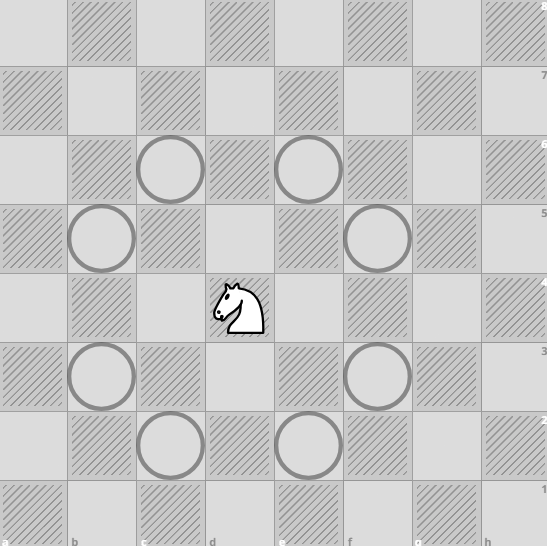
\includegraphics[scale=0.25]{images/centralKnight.png}
    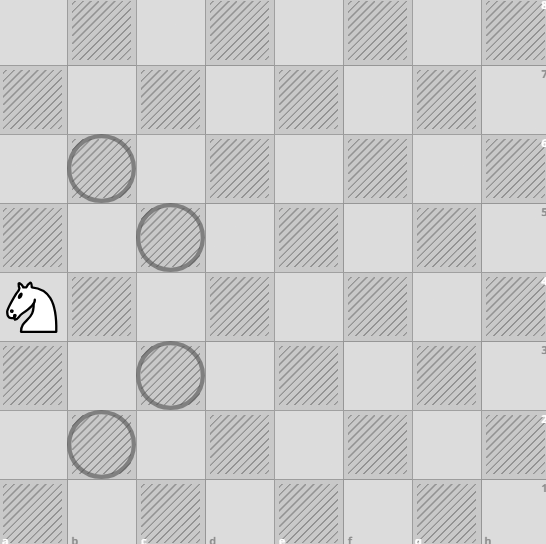
\includegraphics[scale=0.25]{images/rimKnight.png}
    \caption{Spaces controlled by a central Knight vs Spaces controlled by a Knight on the rim}
    \label{fig: knightPositions}
\end{figure}

\begin{figure}[H]
    \centering
    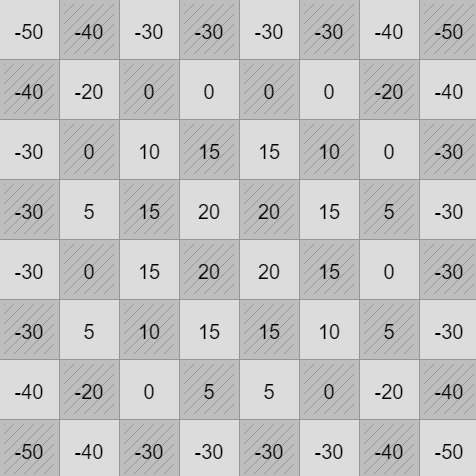
\includegraphics[scale=0.5]{images/KnightSquareValues.png}
    \caption{Piece Square Values for the Knight \cite{pieceSquares}}
    \label{fig:knightPieceSquareVals}
\end{figure}

\subsection{Search}

In order to find the best move in a given position, one must first know what moves are possible to begin with. So naturally one would generate a tree of all possible moves that could branch out of a position within a certain depth. A simple start would be to look at all available moves, three moves deep (Usually a move refers to two plies i.e. a move by white and a move by white. In this context a move refers to a single ply for the sake of simplicity). Figure \ref{minmax} shows how the tree would look.

As mentioned before, chess has quite a large branching factor, meaning at any point of time during a game, the number of possible positions that increases exponentially. Table \ref{tab:posTable} quantifies this fact for the first few moves of a game. Due to that, it would not only be counterproductive to generate all possible moves from a position, but outright impossible. To solve this, analysing how humans play chess (more specifically how Grandmasters play) provide a useful perspective to improving the search function.

\begin{table}[H]
    \centering
    \begin{tabular}{ ||c c|| } 
      \hline
      Number of plies (half-moves) & Number of possible positions\\ 
      \hline\hline
      1 & 20 \\ 
      \hline
      2 & 400 \\
      \hline
      3 & 8902 \\
      \hline
      4 & 197281 \\
      \hline
      5 & 4865609 \\
      \hline
    \end{tabular}
    \caption{Possible positions with each move}
    \label{tab:posTable}
\end{table}

\subsubsection{MinMax}
MinMax is an approach that can be applied to any 2 player game, and not just chess. There's a \textit{Minimising} player and a \textit{Maximising} player, given an evaluation function, a specific position, and whether we're minimising or maximising, we can then follow the procedure described below \cite{Klein}

\begin{itemize}
    \item We create a move tree, where from a root position (in this example we assume the root position is after white made a move) we consider all possible replies. We do the same for each of those replies.
    \item After a certain predetermined depth this process is halted (or earlier due to lack of legal moves, checkmates or draws). This is done in consideration to the limited time and storage resource, and how fast the tree can grow.
    \item From there each leaf node of the tree is evaluated. Positions where white won would have an evaluation of $\infty$, ones where black wins would have -$\infty$ and ones that are drawn would have an evaluation of 0.
    \item These results are then propagated back to the root, so given a position where all child nodes are evaluated we do the following
        \begin{itemize}
            \item take the \textbf{maximum} of all child node evaluations if it's white to play
            \item take the \textbf{minimum} of all child node evaluations if it's black to play
        \end{itemize}
\end{itemize}

The following figure shows the outcome of following the aforementioned steps, keeping in mind that the moves considered here are mostly piece captures, and alongside that the evaluation function used just sums up the value of the pieces.

\begin{figure}[h]
    \centering
    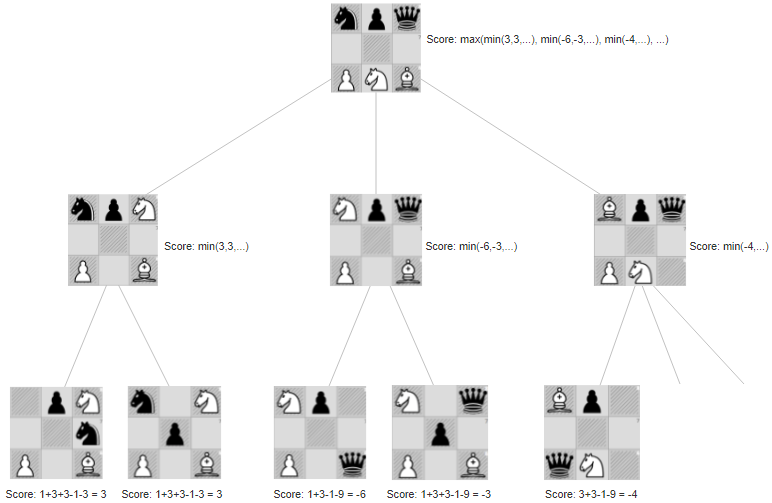
\includegraphics[scale=0.45]{images/minMaxscored.png}
    \caption{Simplified example of MinMax}
    \label{minmax}
\end{figure}

\subsubsection{Alpha-Beta Pruning}

The use of MinMax on its own is effective but comes with the significant drawback of requiring a drastic amount of space and computer power to be able to evaluate each and every possible move, and as mentioned before this would mean that the algorithm would need to evaluate quite a large number of positions depending on the branching factor of a certain position.

To combat this issue Alpha-Beta Pruning was introduced. As the name suggests it \textit{prunes} or cuts off branches that we no longer need to consider. 

Consider that we are deep in our move tree, and white is to move. Assuming we have 2 Nodes, \textbf{Node 1} \& \textbf{Node 2}, and each one of them has 3 child nodes. Assume we then evaluate each child node of Node 1 and back propagate them so that now Node 1 has an evaluation of \textbf{+2}.

When evaluating the first child of Node 2 we come across an evaluation of 6, so now we know that Node 2 would have an evaluation of \textit{at least} 6. At this point we can say that Node 1 has an evaluation of +2 and Node 2 has an evaluation of $\geq+5$. But we know that in the turn that precedes Node 1 and Node 2, it was black's turn to move, and black would try to minimise the score and thus choose Node 1. With that information we can now confidently say that looking further into the children of Node 2 is no longer necessary and prune those branches off.

Figure \ref{minAB} \cite{Klein} shows the application Alpha-Beta Pruning alongside the MinMax algorithm, its application on figure \ref{minmax}

\begin{figure}[h]
    \centering
    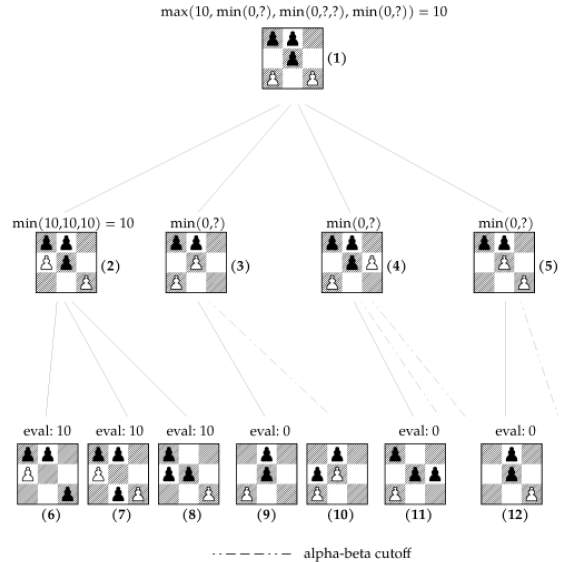
\includegraphics[scale=0.45]{images/kleinPruneFig.png}
    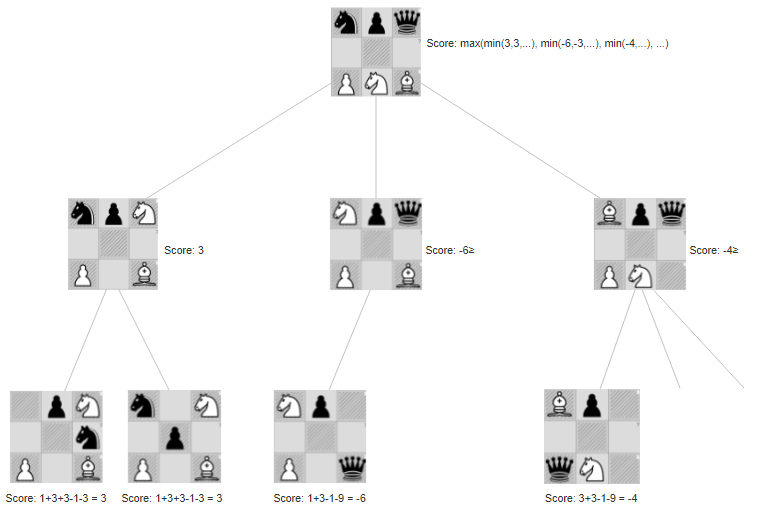
\includegraphics[scale=0.40]{images/minMaxpruned.png}
    \caption{Simplified examples of MinMax \& Alpha-Beta Pruning}
    \label{minAB}
\end{figure}


\subsubsection{Move ordering}
In section \ref{subsubsec: Heuristics} it was mentioned that candidate moves are the ones that have priority when looking for the best move in a position. This means that generating moves that satisfy or follow certain heuristics and evaluating them first would lead to a quicker termination of the search function.

This can be done using some form of a priority queue. An example of this is made clear with table \ref{tab:heuristicPriorityTable}

\begin{table}[H]
    \centering
    \begin{tabular}{ ||c c|| } 
      \hline
      Heuristic & Priority in move list\\ 
      \hline\hline
      Captures & 10 \\ 
      \hline
      Checks & 5 \\
      \hline
      Remaining moves & 0 \\
      \hline
    \end{tabular}
    \caption{Priority of heuristics used to order the moves for searching}
    \label{tab:heuristicPriorityTable}
\end{table}


The aforementioned techniques provide a solid base for most chess engines. They can be used for most types of positions that can arise within a game of chess. In the following sections, these techniques alongside several other ideas as discussed explicitily within the context of chess endgames.